\documentclass{article}\usepackage[]{graphicx}\usepackage[]{color}
%% maxwidth is the original width if it is less than linewidth
%% otherwise use linewidth (to make sure the graphics do not exceed the margin)
\makeatletter
\def\maxwidth{ %
  \ifdim\Gin@nat@width>\linewidth
    \linewidth
  \else
    \Gin@nat@width
  \fi
}
\makeatother

\definecolor{fgcolor}{rgb}{0.345, 0.345, 0.345}
\newcommand{\hlnum}[1]{\textcolor[rgb]{0.686,0.059,0.569}{#1}}%
\newcommand{\hlstr}[1]{\textcolor[rgb]{0.192,0.494,0.8}{#1}}%
\newcommand{\hlcom}[1]{\textcolor[rgb]{0.678,0.584,0.686}{\textit{#1}}}%
\newcommand{\hlopt}[1]{\textcolor[rgb]{0,0,0}{#1}}%
\newcommand{\hlstd}[1]{\textcolor[rgb]{0.345,0.345,0.345}{#1}}%
\newcommand{\hlkwa}[1]{\textcolor[rgb]{0.161,0.373,0.58}{\textbf{#1}}}%
\newcommand{\hlkwb}[1]{\textcolor[rgb]{0.69,0.353,0.396}{#1}}%
\newcommand{\hlkwc}[1]{\textcolor[rgb]{0.333,0.667,0.333}{#1}}%
\newcommand{\hlkwd}[1]{\textcolor[rgb]{0.737,0.353,0.396}{\textbf{#1}}}%

\usepackage{framed}
\makeatletter
\newenvironment{kframe}{%
 \def\at@end@of@kframe{}%
 \ifinner\ifhmode%
  \def\at@end@of@kframe{\end{minipage}}%
  \begin{minipage}{\columnwidth}%
 \fi\fi%
 \def\FrameCommand##1{\hskip\@totalleftmargin \hskip-\fboxsep
 \colorbox{shadecolor}{##1}\hskip-\fboxsep
     % There is no \\@totalrightmargin, so:
     \hskip-\linewidth \hskip-\@totalleftmargin \hskip\columnwidth}%
 \MakeFramed {\advance\hsize-\width
   \@totalleftmargin\z@ \linewidth\hsize
   \@setminipage}}%
 {\par\unskip\endMakeFramed%
 \at@end@of@kframe}
\makeatother

\definecolor{shadecolor}{rgb}{.97, .97, .97}
\definecolor{messagecolor}{rgb}{0, 0, 0}
\definecolor{warningcolor}{rgb}{1, 0, 1}
\definecolor{errorcolor}{rgb}{1, 0, 0}
\newenvironment{knitrout}{}{} % an empty environment to be redefined in TeX

\usepackage{alltt}
\usepackage{amsmath,amsfonts,bm,fullpage,multirow,animate}
\usepackage{natbib,tikz}
\bibliographystyle{abbrvnat}
\DeclareMathOperator*{\argmax}{arg\,max}
\newcommand{\ProjMean}{{\widehat{\bm S}_{2}}}
\newcommand{\ProjMedian}{{\widehat{\bm S}_{1}}}
\newcommand{\HuberMean}{{\widehat{\bm S}_H}}
\newcommand{\WeightMean}{{\widehat{\bm S}_W}}
\newcommand{\TrimMean}{{\widehat{\bm S}_T}}
\newcommand{\WinzMean}{{\widehat{\bm S}_Z}}
\newcommand{\R}{{\mathbb{R}}}
\IfFileExists{upquote.sty}{\usepackage{upquote}}{}
\begin{document}

\begin{center}
\Large{\bf Robustifying the Projected Mean}
\end{center}
\normalsize
This is the literature I have found methods to robustify the $L_2$ estimator for various data types.  Specifically I focus on the trimmed and winsorized means.



 
\section{Trimmed Means}

Assume the sample of size $n$, $x_1,\dots,x_n$, has empirical distribution function $F_n$.  The sample $\alpha$-trimmed mean, according to \cite{huber2009} page 10, is
\[
\bar{X}_\alpha=\frac{1}{1-2\alpha}\int_{\alpha}^{1-\alpha}F_n^{-1}(t)dt.
\]

The following is taken from Section 4 of \cite{laha2011}. In the circular context, suppose $\theta$ is a circular random variable with p.d.f.~$f(\theta)$ and $0<\gamma\leq 0.5$ is fixed.  Let $\alpha,\beta$ be two points on the unit circle satisfying
\[
\int_{\beta}^\alpha f(\theta)d\theta=1-2\gamma.
\] 
The circular $\gamma$-trimmed mean is
\[
\mu_\gamma=\text{arg}\left[\frac{1}{1-2\gamma}\int^{\alpha}_\beta\exp(\imath\theta)f(\theta)d\theta\right].
\]
In their Theorem 4.1 they show it is SB-robust for the circular von Mises distribution.  In \cite{laha2013} they show it is SB-robust for the wrapped normal distribution too.  Remember SB-robustness is always with respect to some dispersion measure.


To define the $SO(3)$ trimmed mean we need to determine which observations are in the tails.  To do this consider the the discordant measure $H_i$ proposed by \cite{best1986} and later expanded to the hypersphere by \cite{figueiredo2005} defined as 
\begin{equation}\label{eqn:Hj}
H_j=(n-2)\frac{1+\hat\tau_{3,j}-\hat\tau_3}{n-1-\hat\tau_{3,j}}
\end{equation}
where $n$ is the sample size, $\hat{\tau}$ is the largest eigenvalue of $T=\sum_{i=1}^n\bm q_i\bm q_i^\top$ and $\hat\tau_{3,i}$ is the largest eigenvalue of $T-\bm q_j\bm q_j^\top$.  See ``Ouliers.pdf" for an expanded discussion on $H_i$.

It follows that $\alpha$-trimmed mean in $SO(3)$ is defined by
\[
\bm S_{T}=\frac{1}{|\Omega_0|}\int_{\Omega_0}\bm Rf(\bm R|\bm S,\kappa)d\bm R
\]
where $\Omega_0=\{\bm R:\bm R\in SO(3), H(\bm R)\leq q_{\alpha}\}$ and $q_\alpha$ is the $100(1-\alpha)\%$ of the distribution of $H_j$.  In practice $\bm S_T$ can be estimated by
\[
\TrimMean=\argmax_{\bm S\in SO(3)}\text{tr}(\bm S^\top\overline{\bm R}_T)
\]
where $\overline{\bm R}_T=\sum_{i=1}^n\bm R_iI(\bm H_i\leq \hat q_{\alpha})$ and $\hat q_{\alpha}$ is the $100(1-\alpha)\%$ of the distribution of $H_i$.




\section{Weighted Means}

According to \cite{huber2009} Section 11.2.2 the current best possible break down for a $d$-dimensional affine equivalent estimator is
\[
\epsilon^*=\frac{n-2d+1}{2n-2d+1}.
\]
So for us, this would be $(n-5)/(2n-5)$.  This break-down is achieved by the weighted average of the points $\bm x_i$ from $\bm X$ with weights $w_i=w(r_i)$ where
\[
r_i=\sup_{\bm u}\frac{\bm u^\top\bm x_i-\text{MED}(\bm u^\top\bm X)}{\text{MAD}(\bm u^\top\bm X)}
\]
and $w(r)$ is a strictly positive, decreasing function of $r\geq 0$, with $w(r)r$ bounded.  I think $r_i$ can be replaced with any one-dimensional projection of the outlyingness of the $\bm x_i$.  

Define the $SO(3)$ weighted mean as
\begin{align*}
\WeightMean=\argmax_{\bm S\in SO(3)}\text{tr}(\bm S^\top\overline{\bm R}_W)
\end{align*}
where $\overline{\bm R}_W=(\sum_{i}w_i\bm R_i)/(\sum_i w_i)$, the weights $w_i^{-1}=\sqrt{H_i}/(\sum_i \sqrt{H_i})$ and $H_i$ is from \eqref{eqn:Hj}.  I use the square root of $H_i$ because $H_i$ alone behaves like a square loss function instead of an absolute loss function.







\section{Huber Estimator \& Winsorized Mean}

The idea of the multidimensional Huber estimator is to robustify an esimator by placing a bound on the norm of its influence function.  In Figure \ref{fig:Huber} the 2-dimensional case is illustrated for the artificial data $\bm q_1,\dots,\bm q_6$.
\begin{figure}
\begin{center}
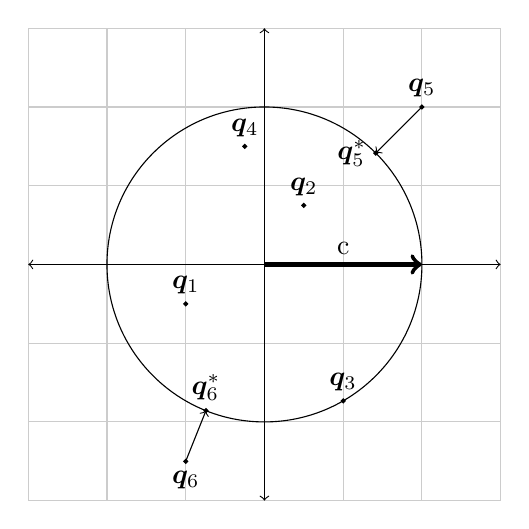
\begin{tikzpicture}
    \draw [black!20] (-3,-3) grid (3,3);
    \draw (0,0) circle [radius=2];
    \draw [->,ultra thick] (0,0) -- (2,0);
    \draw [<->] (-3,0) -- (3,0);
    \draw [<->] (0,-3) -- (0,3);
    %\node [above] at (3,0) {$x$}
    \node [above] at (1,0) {c};
    \node [above] at (-1,-.5) {$\bm{q}_1$};
    \draw [fill] (-1,-.5) circle [radius=0.025];
    \node [above] at (.5,.75) {$\bm{q}_2$};
    \draw [fill] (.5,.75) circle [radius=0.025];
    \node [above] at (1,-1.732051) {$\bm{q}_3$};
    \draw [fill] (1,-1.732051) circle [radius=0.025];
    \node [above] at (-.25,1.5) {$\bm{q}_4$};
    \draw [fill] (-.25,1.5) circle [radius=0.025];
    \node [above] at (2,2) {$\bm{q}_5$};
    \draw [fill] (2,2) circle [radius=0.025];
    \node [left] at (1.414214, 1.414214) {$\bm{q}_5^*$};
    \draw [fill] (1.414214, 1.414214) circle [radius=0.025];
    \draw [->] (2,2) -- (1.414214, 1.414214);
    \node [below] at (-1,-2.5) {$\bm{q}_6$};
    \draw [fill] (-1,-2.5) circle [radius=0.025];
    \node [above] at (-0.7427814,  -1.8569534) {$\bm{q}_6^*$};
    \draw [fill] (-0.7427814, -1.8569534) circle [radius=0.025];
    \draw [->] (-1,-2.5) -- (-0.7427814,  -1.8569534);
\end{tikzpicture}
\end{center}
\caption{Multidimensional Huber estimator as illustrated in Section 4.3 of \cite{hampel2011}.}
\label{fig:Huber}
\end{figure}

Each point represents the influence function evaluated at that data point.  The norm of the influence function for this estimator evaluated at $\bm q_1,\dots,\bm q_4$ all lie within the specified distance of the origin so they are left untouched.  The norm of the influence function evaluated at $\bm q_5$ and $\bm q_6$ however is larger than $c$ and therefore those points are altered such that the norm of the influence function has a norm of $c$.  The reason (according to pp 239 of \citealt{hampel2011}) for placing the bound on the influence function is because  ``the most meaningful version of the $\psi$-function defining an $M$-estimator is its influence function."

Applying this idea to $SO(3)$ data, recall from the regions paper that the influence function of $\ProjMean$ is
\[
\text{IF}_2(\bm R_i,F)=\frac{3}{1+2E[\cos(r)]}\sin(r)\bm u
\]
where $r=d_r(\bm R_i,\bm S)$ or in practice $\hat{r}=d_r(\bm R_i,\ProjMean)$.  It follows that $\|\text{IF}_2(\bm R_i,F)\|\propto \sin(|r|)$.  Unfortunately, using the Huber estimator directly will put the most restrictions on the $r$ values near $\pi/2$ instead or $\pi$, which is where we really want to place the upper bound.  Therefore I propose the modified Huber estimator on $SO(3)$ put a bound on $r_i=d_r(\bm R_i,\ProjMean)$ and is denoted $\HuberMean$.  

The algorithm I use to compute $\HuberMean$ based on the sample $\bm R_1,\dots,\bm R_n$ and the constant $c<\pi$ is as follows
\begin{enumerate} 
\item Compute $\ProjMean^{(j)}$
\item For each $i$ compute $r_i^{(j)}=d_r(\bm R_i,\ProjMean^{(j)})$
\item For each $i$ such that $r_i>c$:
\begin{enumerate}
\item Find $\bm u_i\in\mathcal{S}^3$ satisfying $\exp[\bm{\Phi}(r_i\bm u_i)]=\ProjMean^{(j)\top}\bm R_i$
\item Redefine $\bm R_i=\ProjMean^{(j)\top}\exp[\bm{\Phi}(c\bm u_i)]$
\end{enumerate}
\item Repeat steps 1 - 3 for $j+1$ until $r_i<c$ for all $i$
\item Define $\HuberMean=\ProjMean^{(j+1)}$
\end{enumerate}

The winsorized mean is a combination of the trimmed mean and winsorized mean.  That is, the data are ordered according to their respective $H_j$ values.  All rotations beyond the upper $100(1-\alpha)$\% percentage is projected to the border of the inner circle while maintaining the original axis of rotation.  The mathematical definition is 
\[
\WinzMean=\argmax_{\bm S\in SO(3)}\text{tr}(\bm S^\top\overline{\bm R}_{Z})
\]
where $\overline{\bm R}_{Z}=\sum_{i=1}^n\bm R_i^*/n$, 
\[
\bm R_i^*=
\begin{cases}
\bm R_i&\text{ if }d_R(\ProjMean,\bm R_i)\leq\hat{q}\\
\ProjMean\exp[\bm{\Phi}(\hat{q}\bm{u}_i^*)]&\text{ otherwise,}
\end{cases}
\]
$\bm u_i^*$ is the axis of rotation corresponding to $\ProjMean^\top\bm R_i$ and $\hat{q}$ is the $100(1-\alpha)$\% percentile of the distribution of $H_j$.


% 
% Thus the gross error sensitivity is
% \[
% \|\text{IF}_2(\bm R_i,F)\|=\|\frac{3}{1+2E[\cos(r)]}\sin(r)\bm u\|=\left|\frac{3\sin(r)}{1+2E[\cos(r)]}\right|=\frac{3\sin(|r|)}{1+2E[\cos(r)]}
% \]

\begin{knitrout}
\definecolor{shadecolor}{rgb}{0.969, 0.969, 0.969}\color{fgcolor}











{\centering \animategraphics[width=.5\textwidth,controls,loop]{1}{Figure/huberContd}{1}{11}

}



\end{knitrout}









\section{(Very) Limited Simulation Study}

I ran a very small simulation study with the new robustified $\ProjMean$ estimators (trimmed, winsorized, weighted, Huber) along with the tradition $\ProjMean$ and $\ProjMedian$.  I generated 100 samples per combination of distribution (Cayley or von Mises Fisher), sample size ($n=10,50$), concentration ($\kappa=0.5,1,10$) all with $10\%$ contamination.  Meaning 90\% of each sample was from the $F(\bm I_{3\times 3},\kappa)$ distribution and 10\% of the sample came from a $F(\bm S_c[\pi/2,\bm u],\kappa)$, i.e.~the slippage situation where the second principal direction was rotation though $\pi/2$ radians about some (uniformly distributed) axis.

In Table \ref{tab:SimResHn} is the average bias based on the Euclidean distance in each estimator for each simulated scenario.  That is bias$=\|\bm I_{3\times 3}-\widehat{\bm S}\|_F$ for each estimator.  The trimmed and winsorized mean use $\alpha=0.1$ and the Huber estimator sets $c=0.75$.





% \begin{table}[ht]
% \centering
% \begin{tabular}{lrrrrrrrr}
%   \hline
%   Dist& n & $\kappa$  & Mean & Median & Trim & Winz & Weight &Huber\\ 
%   \hline
%   & &0.50  & 1.46 & 1.64 & 1.52 & 1.45 & 1.51 & 1.45 \\
%   & 10&1.00  & 1.06 & 1.30 & 1.11 & 1.04 & 1.15 & 1.05 \\ 
%  \multirow{2}{*}{Cayley} & &10.00  & 0.35 & 0.38 & 0.35 & 0.36 & 0.35 & 0.35 \\ \cline{2-9}
%   & &0.50 & 0.81 & 0.97 & 0.85 & 0.77 & 0.87 & 0.78 \\ 
%   & 50&1.00  & 0.51 & 0.64 & 0.53 & 0.47 & 0.56 & 0.49 \\
%   & &10.00 & 0.21 & 0.18 & 0.16 & 0.20 & 0.19 & 0.19 \\ \hline
%   
%   & &0.50 & 0.70 & 0.48 & 0.72 & 0.71 & 0.58 & 0.69 \\ 
%   & 10&1.00  & 0.49 & 0.32 & 0.52 & 0.51 & 0.38 & 0.46 \\
%  \multirow{2}{*}{von Mises} & &10.00& 0.20 & 0.09 & 0.14 & 0.18 & 0.12 & 0.17 \\ \cline{2-9}
%   & &0.50   & 0.30 & 0.14 & 0.31 & 0.31 & 0.20 & 0.29 \\ 
%   & 50&1.00 & 0.27 & 0.11 & 0.28 & 0.27 & 0.17 & 0.25 \\ 
%   & &10.00 & 0.17 & 0.03 & 0.06 & 0.12 & 0.07 & 0.12 \\
%    \hline
% \end{tabular}
% \caption{Mean estimator bias based on 100 samples from each combination of distribution, sample size and concentration.}
% \label{tab:SimRes}
% \end{table}

\begin{table}[ht]
\centering
\begin{tabular}{l|lll|lll|lll|lll}
  \hline
 & \multicolumn{6}{|c|}{Cayley} & \multicolumn{6}{|c}{von Mises}   \\ 
\hline
   &  \multicolumn{3}{|c|}{n=10} & \multicolumn{3}{|c|}{n=50} & \multicolumn{3}{|c|}{n=10} & \multicolumn{3}{|c}{n=50} \\ 
  $\kappa$ &  0.5 &  1.0 & 10.0 &  0.5 &  1.0 & 10.0 &  0.5 &  1.0 & 10.0 &  0.5 &  1.0 & 10.0 \\ \hline
  $\ProjMedian$ (Median) & 1.71 & 1.30 & 0.37 & 0.92 & 0.66 & 0.18 & 0.52 & 0.33 & 0.09 & 0.15 & 0.11 & 0.03 \\ 
  $\ProjMean$ (Mean) & 1.55 & 1.10 & 0.35 & 0.79 & 0.55 & 0.21 & 0.66 & 0.49 & 0.20 & 0.31 & 0.23 & 0.17 \\ 
  $\TrimMean$ (Trim) & 1.56 & 1.16 & 0.34 & 0.80 & 0.57 & 0.16 & 0.70 & 0.52 & 0.13 & 0.33 & 0.24 & 0.06 \\ 
  $\WinzMean$ (Winsorize)& 1.56 & 1.11 & 0.36 & 0.75 & 0.51 & 0.21 & 0.68 & 0.51 & 0.18 & 0.32& 0.24 & 0.12 \\ 
  $\WeightMean$ (Weight) & 1.61 & 1.17 & 0.36 & 0.84 & 0.60 & 0.19& 0.56 & 0.39 & 0.12 & 0.21 & 0.15 & 0.07\\ 
  $\HuberMean$ (Huber) & 1.55 & 1.11 & 0.35 & 0.77 & 0.54 & 0.20 & 0.65 & 0.47 & 0.17 & 0.30 & 0.22 & 0.13 \\ 
   \hline
\end{tabular}
\caption{Mean estimator bias based on 100 samples from each combination of distribution, sample size and concentration.  The robustified $L_2$ estimator is based on the distance of the observations from the bulk of the data, quanitifed by the $H_n$ statistic.}
\label{tab:SimResHn}
\end{table}

\begin{table}[ht]
\centering
\begin{tabular}{l|lll|lll|lll|lll}
  \hline
 & \multicolumn{6}{|c|}{Cayley} & \multicolumn{6}{|c}{von Mises}   \\ 
\hline
   &  \multicolumn{3}{|c|}{n=10} & \multicolumn{3}{|c|}{n=50} & \multicolumn{3}{|c|}{n=10} & \multicolumn{3}{|c}{n=50} \\
  $\kappa$ &  0.5 &  1.0 & 10.0 &  0.5 &  1.0 & 10.0 &  0.5 &  1.0 & 10.0 &  0.5 &  1.0 & 10.0 \\ \hline
  $\ProjMedian$ (Median) & 1.70 & 1.25 & 0.35 & 1.01 & 0.59 & 0.19 & 0.55 & 0.37 & 0.08 & 0.15 & 0.11 & 0.03 \\ 
  $\ProjMean$ (Mean) & 1.56 & 1.04 & 0.33 & 0.83 & 0.49 & 0.22 & 0.76 & 0.50 & 0.19 & 0.30 & 0.25 & 0.17 \\ 
   $\TrimMean$ (Trim) & 1.68 & 1.12 & 0.34 & 0.86 & 0.52 & 0.17 & 0.82 & 0.53 & 0.13 & 0.31 & 0.23 & 0.06 \\ 
  $\WinzMean$ (Winsorize) & 1.60 & 1.06 & 0.34 & 0.82 & 0.49 & 0.18 & 0.74 & 0.51 & 0.13 & 0.29 & 0.22 & 0.06 \\ 
  $\WeightMean$ (Weight) & 2.07 & 1.52 & 0.33 & 2.06 & 0.83 & 0.20 & 1.37 & 0.74 & 0.12 & 0.75 & 0.41 & 0.08 \\ 
  $\HuberMean$ (Huber) & 1.56 & 1.03 & 0.33 & 0.82 & 0.48 & 0.20 & 0.74 & 0.49 & 0.16 & 0.28 & 0.23 & 0.13 \\ 
   \hline
\end{tabular}
\caption{Mean estimator bias based on 100 samples from each combination of distribution, sample size and concentration.  The robustified $L_2$ estimator is based on the influence of the point on the $L_2$ estimator, quanitifed by the influence function.}
\label{tab:SimResC}
\end{table}




\begin{figure}
\centering
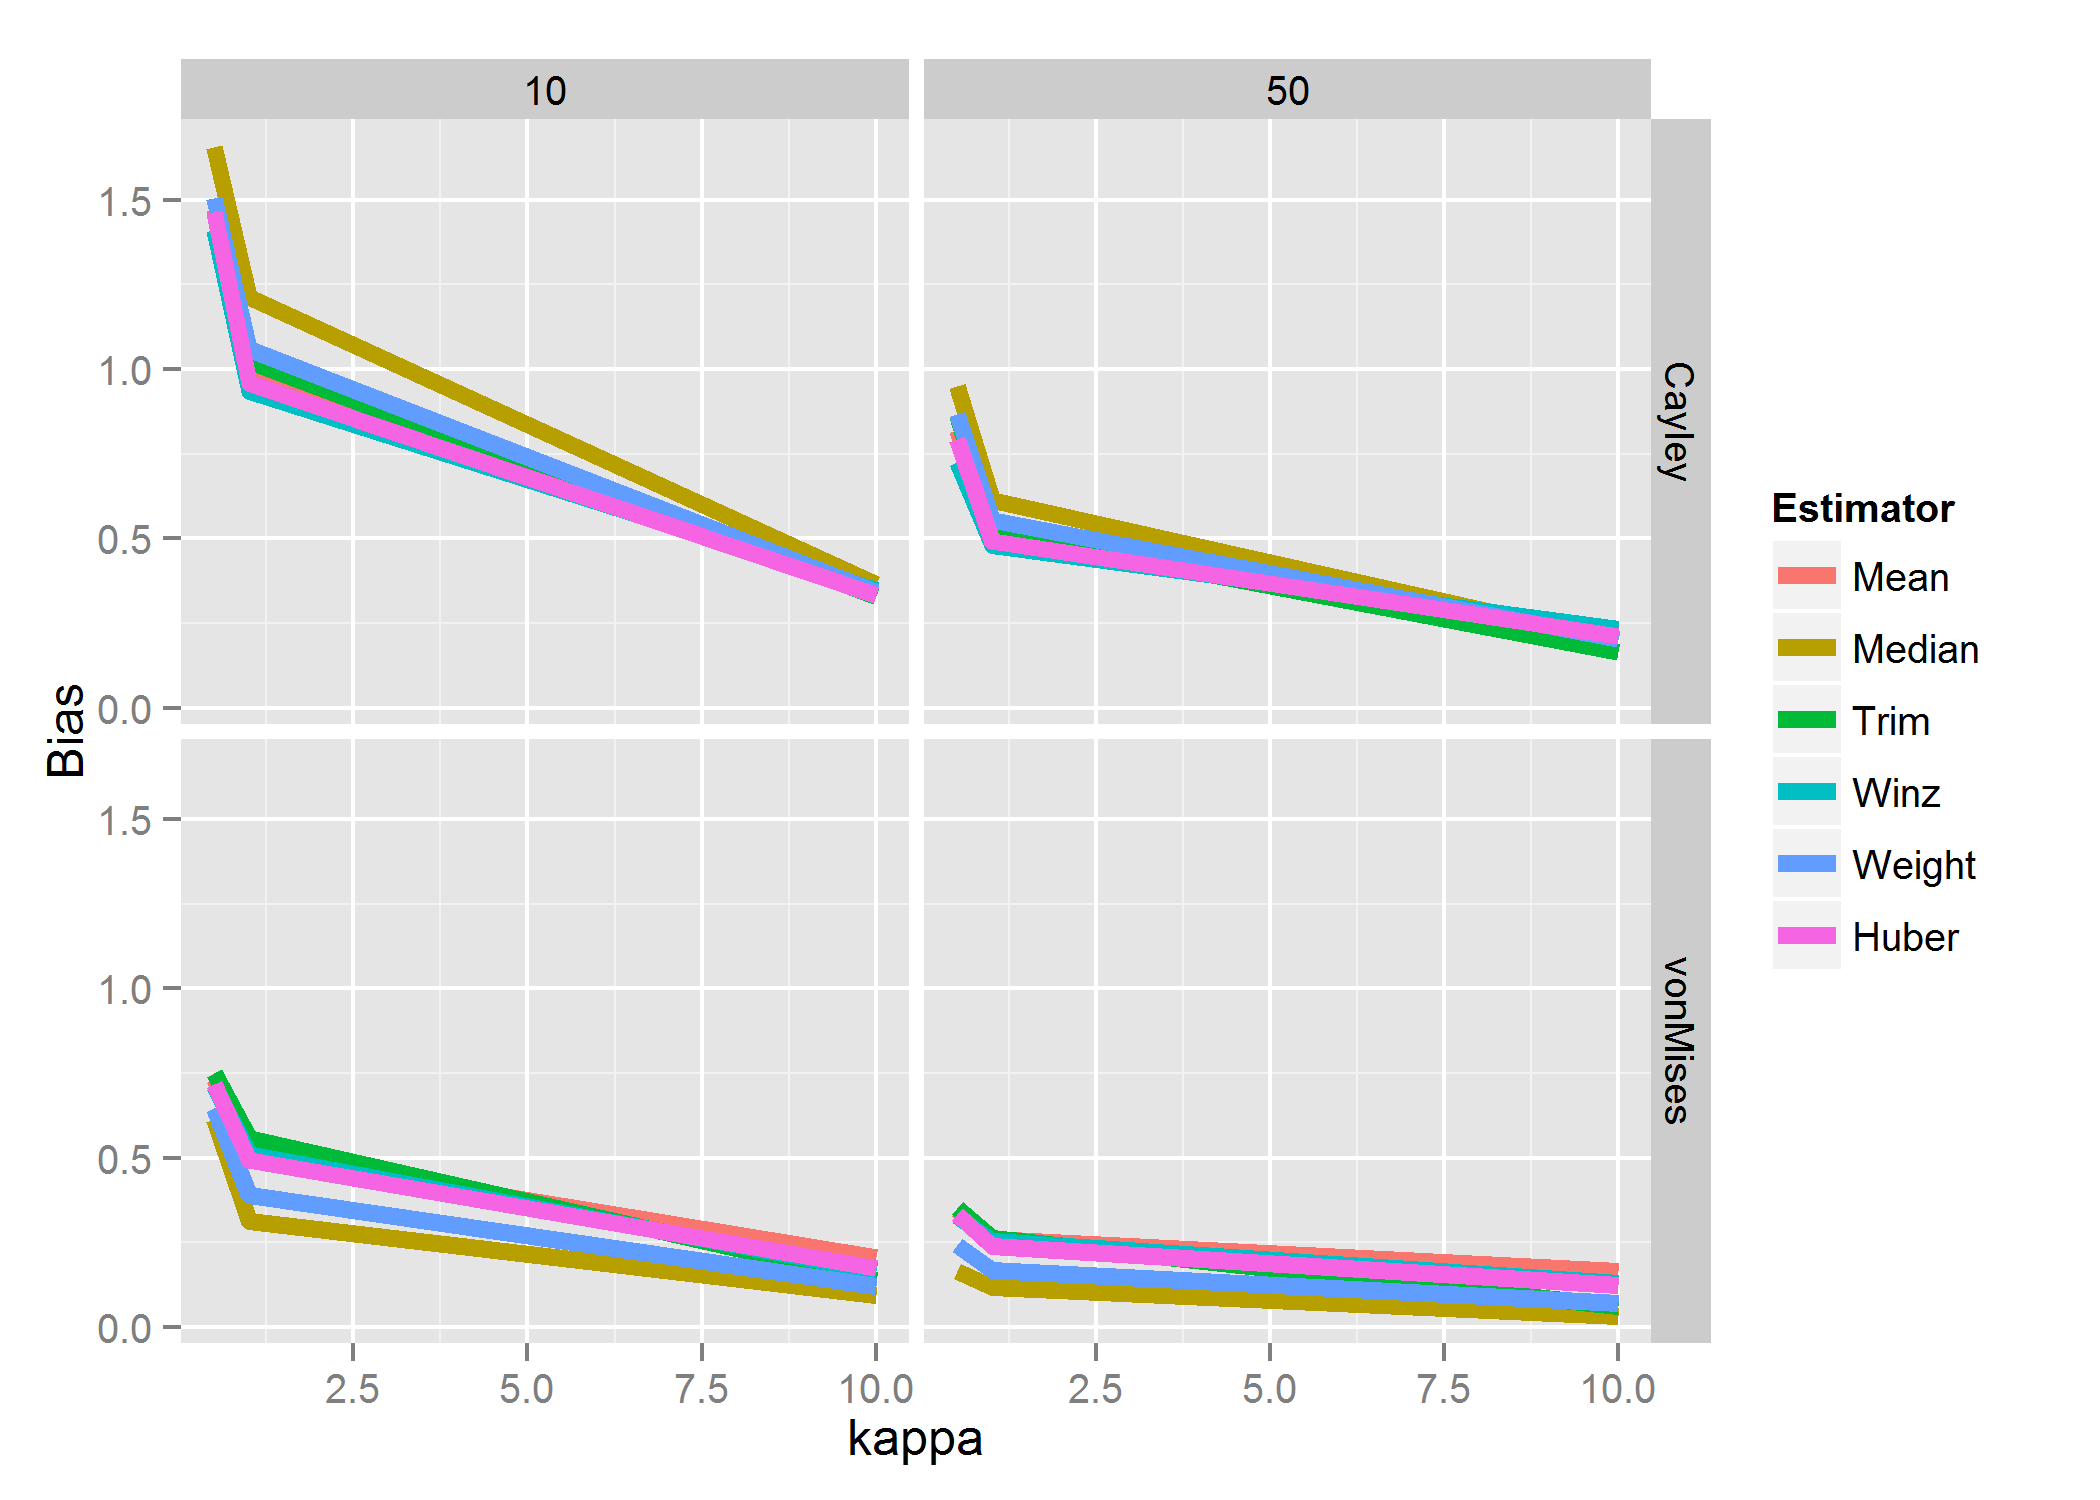
\includegraphics[width=.7\textwidth]{Estimator.png}
\caption{Graphical representation of Table \ref{tab:SimResHn} faceted by sample size and distribution.}
\end{figure}


For the Cayley (and presumably Fisher matrix) distribution, the Huber estimator and trimmed mean are close.  Trimmed mean is preferred for more concentrated data and the Huber estimator is preferred as the data become less concentrated.  This makes sense because the trimmed mean is discarding the contaminated data when the bulk of the data is highly concentrated, while the Huber estimator is trying to use all the data.  The median does really poorly, even compared to the mean.

For the von Mises distribution, it looks like the median is unbeatable.  This is likely due to the heavy tail we identified in the Technometrics paper.  Similar to the other distribution, the trimmed mean improves considerably as the bulk of the data becomes more concentrated and the contamination can be cut out completely.  The Huber estimator and winsorized mean give comparable results but are not terribly good.
\clearpage
%\bibliographystyle{plain}
\bibliography{../OutlierDetection/RobustRefs}
\end{document}
